\startchapter{Channel Modeling}
\label{chapter:Mod}
In this section, I modeled communication in the traces. Then I investigated 4 different channel types: Named pipes, MQMS, TCP/UDP socket and HTTP channels, all of which are the most fundamental ones in Windows communication framework. By matching these channels to the communication model I verified generality of the modeling. 

\section{Communication Modeling}
As defined before, a communication event in the dual-trace is defined as message send and received in a specific channel. In the assembly trace level, we have to be able to locate the send or receive function calls of a specific channel in both side of the traces and then retrieve the message from the memory change recorded in the trace. 
\subsection{How Communications Happen}   
A communication in this work is happen in a channel. There are 3 main stages of a communication in this model: 1. create/open the channel, 2. message send/receive, 3. delete/close the channel. Some channel may have several step in each stage. Figure \ref{communicationhappen}. In the create/open channel stage, each end may need to call its own channel create or open functions. For some channel type multiple open/create/connect functions might be called to finish the task. In the message send/receive stage, messages are being sent into the channel in one side and received in the other side. In the final channel delete/close stage, the channel delete or close functions will be called to finish the task. The closed channel can be reopen again to continue the communication.
\begin{figure}[h]
\centerline{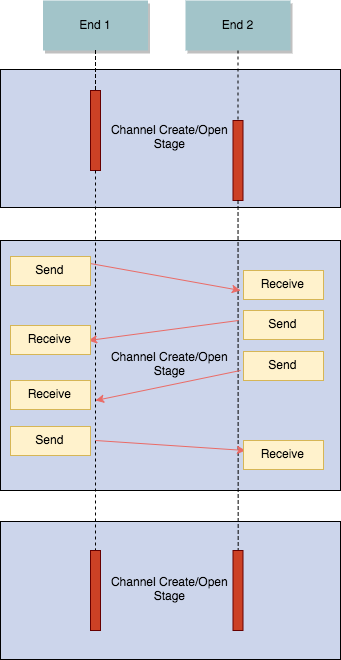
\includegraphics[scale=0.5]{Figures/communicationhappen}}
 \caption{Three main stage of the communication between two ends of a channel}
\label{event}
\end{figure}

\subsection{Scenarios}
There are many scenarios of the communication. It can be success or fail. The message can be lost. The sent message can be broken into several sub-messages and the receiver may receive several sub-messages instead of a whole one. Or several sent message will be receive once in the receiver side. Or even more complicated, the messages are reconstruction in the channel and reach the receiver. 
\begin{enumerate} 
\item There are four operations being concerned in this model: channel open, message send, message receive, and channel close. \item The number of send and receive function calls for one message do not necessary to be the same. It can be one to one, one to multiple, multiple to one, or multiple to multiple.
\item Both sides of the channel shared the same channel name but different channel handle for its own operations.
\item The message send sequence does not necessary the same as the message receive sequence on different sides of the channel.
\end{enumerate} 
\section{Named Pipes Channel}
A named pipe is a named, one-way or duplex pipe for communication between the pipe server and one or more pipe clients. In here we only consider one server V.S one client dual-trace. One server to multiple clients scenario can always be divided into multiple server/client dual-traces. We call the end of the named pipe instance. An instance can be a server instance or a client instance. All instances of a named pipe share the same pipe name, but each instance has its own buffers and handles, and provides a separate conduit for client/server communication. 

A named pipe server responsible for the creation of the pipe, while clients of the pipe can connect to the server after it created. The creation and connection of a named pipe will return the handle ID of that pipe. As we mention before, each instance has its own handles, so the returned handle IDs of the pipe creation function of the server and pipe connection function from each client are different. These handler IDs will be used later on when messages are being sent or received to specify a pipe to which send.


\subsection{Important Channel Parameters}
There are many options for a named pipe. Some of them are critical in the perspective of the channel operations. In this sections we list those ones that are important and affect the strategy of the event locating.
\subsubsection{Buffer Size}
Both the server and client can read or write into the pipe. The pipe server and client can be on the same or different computers. Buffer sizes of server and client can be different. This affect the write/read operation. If the writer's buffer is larger than the reader's buffer and the writer write a message whose size is larger than the reader's buffer. The reader may need to read several times to get the whole message. However, the reader can only read content from a write on the other side of the pipe. This means that even the buffer of the reader is big enough to hold several message from the other side, one read operation will only read the content from one write operation of the other side. And the sequence of the message do not change from the writer side to the reader side. Figure \ref{event} shows the operation scenarios of the write/read operation of the named pipe.

\begin{figure}[h]
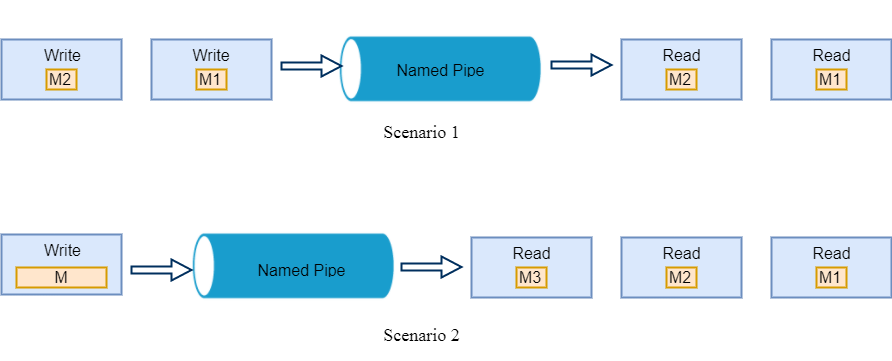
\includegraphics[scale=.48]{Figures/event}
 \caption{write/read operation scenarios: Scenario 1. The written message can fit in the Reader's buffer. The order of the message going into the pipe is the same as the order going out of the pipe; Scenario 2. The written message size is larger than the Reader's buffer, so the read use multiple read operation to receive one message.}
\label{event}
\end{figure}

\subsubsection{Blocking/Non-Blocking}
The named pipe channel can be opened in blocking mode or non-blocking mode. In blocking mode, when the pipe handle is specified in the ReadFile, WriteFile, or ConnectNamedPipe function, the operations are not completed until there is data to read, all data is written, or a client is connected. In non-blocking mode, ReadFile, WriteFile, and ConnectNamedPipe always return immediately. The operation fail if the channel is not ready for read, write or connection. However, since in this work we only aimed at locating the successful communication, as long as the operations success, we can locate them no matter the pipe is in blocking or non-blocking mode.

\subsubsection{Synchronous/Asynchronous}
Another critical option for named pipe channel is Synchronous/Asynchronous. In Synchronous mode, the ReadFile, WriteFile TracnsactNamedPipe and connectNamedPipe functions does not return until the operation it is performing is completed. That means we can retrieve the sent/receive message in the trace when the function return. When the channel is enable overlapped mode, the ReadFile, WriteFile TracnsactNamedPipe and connectNamedPipe functions perform asynchronously. In the asynchronous mode, ReadFile, WriteFile, TransactNamedPipe, and ConnectNamedPipe operations return immediately regardless if the operations are completed. And if the function call return ERROR\_IO\_PENDING, the calling thread then call the GetOverlappedResult function to determine the results. For the read operation, the message will be stored in the buffer indicated in the ReadFile function call when the read operation complete successfully.




\subsection{Function Calls That Consist A Communication Event In The Dual-Trace}
As we talk in the parameters section, Synchrounous and Asychronous mode affect the functions used to complete the send and receive operation as well as the operation of the functions. In the follow subsections, we will list the related functions for the named pipe channel for both synchronous mode and asynchronous mode. The create channel functions for both modes are the same but with different input parameters. The functions for send and receive message are also the same for both case. However, the operation of the send and receive functions are different for different mode. In addition, extra functions are being called to check the status of message sending or receiving in asynchronous mode.
\subsubsection{Synchronous}
We list all the functions that needed to locate an messaging event in a dual-trace in Table\ref{synfunctions} for synchronous named pipe. The Channel Create Functions indicate how the channel being created in server and client sides, and they are different. The file name is an input parameter for CreateNamedPipe and CreateFile function. The client and server of the same pipe use the same file name. This is an important parameter to identify the pipe between the server and client in the traces. The File name is stored in the RCX register when the function is being called. The file handle is a integer return value from the CreateNamedPipe and CreateFile functions call. It will be stored in RAX register when the function return. This handle will be used as the identifier of a pipe in the client or server later on. The handle is different for server and each client even they connected to the same pipe. The send or receive message functions are the same in server and client. the file handle generated when the channel created are stored in register RCX when the WriteFile and ReadFile functions are being called. RDX holds the address of the buffer for message send or receive. The actual size of the message being sent or received are store in R9 when the function return.
  
    \begin{table}[h]
        \centering
        \caption{Functions for communication type definition of synchronous named pipe}
        \label{synfunctions}
        \begin{tabular}{|l|l|l|l|l|}
            \hline
             \multirow{2}{*}{\textbf{Operations}} &
               \multicolumn{2}{c|}{\textbf{Server}} &
               \multicolumn{2}{c|}{\textbf{Client}} \\
             \cline{2-5}
              & \textbf{Function}& \textbf{Parameters} & \textbf{Function} & \textbf{Parameters}  \\
             \hline
             \multirow{2}{*}{\parbox{1.8cm}{\textbf{Channel Create}}}
             &\multirow{2}{*}{\parbox{2.5cm}{CreateNamed- Pipe}} &  RAX: File Handler & \multirow{2}{*}{CreateFile} &  RAX: File Handler\\
              \cline{3-3} \cline{5-5}
             &&  RCX: File Name &  &  RCX: File Name\\
            \hline
             \multirow{3}{*}{\parbox{1.8cm}{\textbf{Message Send}}}
             &\multirow{3}{*}{WriteFile} &  RCX: File Handle & \multirow{3}{*}{WriteFile} &  RCX: File Handle\\
              \cline{3-3} \cline{5-5}
             &&  RDX: Buffer Address &  &  RDX: Buffer Address\\
                           \cline{3-3} \cline{5-5}
             & &  R9: Message Length &  &  R9: Message Length\\
            \hline
            \multirow{3}{*}{\parbox{1.8cm}{\textbf{Message Receive}}}
             & \multirow{3}{*}{ReadFile}&  RAX: File Handle & \multirow{3}{*}{ReadFile} &  RCX: File Handle\\
              \cline{3-3} \cline{5-5}
              &&  RDX: Buffer Address &  &  RDX: Buffer Address\\
                           \cline{3-3} \cline{5-5}
             & &  R9: Message Length &  &  R9: Message Length\\
            \hline
        \end{tabular}
    \end{table}
\subsubsection{Asynchronous}
The functions used in Asynchronous mode for create channel, send and receive message are the same as those used in synchronous mode. However,  the ReadFile and WriteFile functions run asynchronously when the channel is asynchronous. This means the function will return immediately, even if the operation has not been completed. If the operation is complete when the function returns, the return value indicates the success or failure of the operation. Otherwise the functions return zero and GetLastError returns ERROR\_IO\_PENDING. In this case, the calling thread must wait until the operation has finished. The calling thread must then call the GetOverlappedResult function to determine the results. This means besides looking for ReadFile and WriteFile function calls in the traces, the GetOverlappedResult function should be checked in the traces to get the full result of the ReadFile or WriteFile operations. There are two scenarios of the successful communication in the dual-trace for asynchronous mode. The first one is exactly the same as synchronous situation. The second one involves the functions listed in Table\ref{asynfunctions}. In the later one, Read operation searching is bit more complicated, since ReadFile function has to be located first to get the buffer address, and then GetOverlappedResult function return should be search for the message retrieval from the memory.
    \begin{table}[h]
        \centering
        \caption{Functions for additional communication type definition of asynchronous named pipe}
        \label{asynfunctions}
        \begin{tabular}{|l|l|l|l|l|}
            \hline
             \multirow{2}{*}{\textbf{Operations}} &
               \multicolumn{2}{c|}{\textbf{Server}} &
               \multicolumn{2}{c|}{\textbf{Client}} \\
             \cline{2-5}
              & \textbf{Function}& \textbf{Parameters} & \textbf{Function} & \textbf{Parameters}  \\
             \hline
             \multirow{2}{*}{\parbox{1.8cm}{\textbf{Channel Create}}}
             &\multirow{2}{*}{\parbox{2.5cm}{CreateNamed- Pipe}} &  RAX: File Handler & \multirow{2}{*}{CreateFile} &  RAX: File Handle\\
              \cline{3-3} \cline{5-5}
             &&  RCX: File Name &  &  RCX: File Name\\
            \hline
             \multirow{3}{*}{\parbox{1.8cm}{\textbf{Message Send}}}
             &\multirow{3}{*}{WriteFile} &  RCX: File Handle & \multirow{3}{*}{WriteFile} &  RCX: File Handle\\
              \cline{3-3} \cline{5-5}
             &&  RDX: Buffer Address &  &  RDX: Buffer Address\\
                           \cline{3-3} \cline{5-5}
             & &  R9: Message Length &  &  R9: Message Length\\
            \hline

            \multirow{3}{*}{\parbox{1.8cm}{\textbf{Message Receive}}}
             & \multirow{3}{*}{ReadFile}&  RAX: File Handle & \multirow{3}{*}{ReadFile} &  RCX: File Handle\\
              \cline{3-3} \cline{5-5}
              &&  RDX: Buffer Address &  &  RDX: Buffer Address\\
                           \cline{3-3} \cline{5-5}
             & &  R9: Message Length &  &  R9: Message Length\\
                          \hline
            \multirow{2}{*}{\parbox{1.8cm}{\textbf{Status Check}}}
             & \multirow{2}{*}{\parbox{2.5cm}{GetOver- lappedResult}}&  RCX: File Handler & \multirow{2}{*}{\parbox{2.5cm}{GetOver- lappedResult}} &  RCX: File Handler\\
              \cline{3-3} \cline{5-5}
             & &  R8: Message Length &  &  R8: Message Length\\
            \hline
        \end{tabular}
    \end{table}
    
    

\section{MQMS Channel}
\subsection{Synchronous}
\subsection{Asynchronous}

\section{TCP/UDP Socket Channel}
\section{HTTP Channel}


